
\section{Weakly Supervised Semantic Segmentation}
\label{sec:weakly-supervised}
Fully supervised semantic segmentation depends on pixel-level segmentation masks annotated by humans. However, generating such dense annotations is tedious, time-intensive, and costly. Furthermore, crowd-sourced annotators must undergo special training to handle the complexity of pixel-level labeling, which restricts the scale and diversity of available datasets. Consequently, most curated datasets are limited to a small set of object categories. In contrast, unlabeled or weakly annotated images can be collected in abundance, at much lower cost and in shorter time. This has motivated research into weakly supervised semantic segmentation (WSSS) to make semantic segmentation models more scalable.


\section{Types of WSSS}
\label{sec:types-weakly-supervised}
A wide range of weak supervision have been explored, including bounding boxes, scribbles, points, image-level labels,  eye tracks, free-form squiggles, or noisy web tags. Bounding boxes provide rough object boundaries, offering useful localization cues, though they still require annotators to draw accurate boxes.  Scribble-based supervision allows annotators to roughly mark object regions without outlining exact object boundaries. Point supervision, by contrast, typically uses a single annotated pixel per object, giving coarse location information. While less costly than pixel-accurate masks, these methods still involve some level of manual annotation, making large-scale labeling expensive.


\section{Image-level Label based weak supervision}
\label{sec:image-level-label}
Image-level annotation represents a cost-effective and efficient form of supervision for weakly supervised semantic segmentation. Here, each training image is provided only with class labels indicating which object categories are present, but without any information about their spatial locations. The main challenge, therefore, is to correctly associate these image-level labels with the appropriate pixels in the image.

Initial approaches attempted to train segmentation models directly from image-level labels \cite{dcnn}, but performance was unsatisfactory. Later methods introduced discriminative localization techniques such as Class Activation Maps (CAMs) \cite{cam}, which highlight class-relevant regions. These coarse cues were then refined using auxiliary information such as superpixels \cite{imagelevelpixel}, segmentation proposals \cite{imagelevelpixel}, or motion information from videos \cite{wsss_motion_cues}. Some works, such as Adversarial Erasing \cite{adversarial_erasing}, expanded object coverage progressively by iteratively searching new regions. Others, like Kolesnikov and Lampert \cite{kolesnikov2016}, trained networks to approximate the dense CRF \cite{krähenbühl} applied on CAMs for refinement.

Some approaches learn to predict affinity matrices at the pixel level [36], to refine the output of dCRF through random walk. AffinityNet \cite{wsss_affinitynet} predicts class-agnostic pixel affinities to propagate CAM activations via random walks. Similarly, Seeded Region Growing (SRG) \cite{srg} expands initial seed regions using similarity criteria, while its deep learning extension DSRG \cite{wsss_dsrg_deep_seeded_region_growing} leverages high-level semantic features to grow regions more effectively. P2P \cite{pixel_to_prototype} further narrows the supervision gap by using pixel-to-prototype contrastive learning. A common limitation, however, is that most of these CNN-based methods inherit the restricted locality of convolutional features.

Recent advances incorporate transformers into WSSS \cite{camtokens, getam}. TS-CAM \cite{camtokens} leverages the global information capturing ability of ViT by combining class-token attention with CAMs. \cite{getam} refines class-specific maps by using attention gradients. MCTformer \cite{wsss_MCTformer} expands this idea by embedding multiple class tokens to learn attention maps for different categories. AFA \cite{wsss_afa_affinity_from_attention} instead derives semantic affinities directly from attention maps to refine coarse pseudo-labels. FrozenCLIP \cite{wsss_frozen_clip} pushes this further by exploiting the frozen CLIP backbone to generate high-quality pseudo-labels, which are dynamically updated using a refinement module (RFM).


\section{WSSS Training Approaches}
\label{sec:stages}

Weakly supervised semantic segmentation has two main solutions based on their training processes: multi-stage approaches \cite{instance_wsss,wsss_L2G,wsss_rib} and single-stage approaches \cite{wsss_reliability_does_matter, wsss_afa_affinity_from_attention}.

\subsection{Multi Stage}
\label{subsec:multi-stage}

Multi Stage WSSS has multiple steps. Typically, a classification model is first trained to generate the CAM,  which are then converted into initial pixel-level pseudo labels. These pseudo labels are refined through affinity matrix and random walk propagation\cite{wsss_affinitynet, wsss_afa_affinity_from_attention}, or seeded region growing[SRG] or contrastive learning. Then these refined pseudo labels are used for supervising a segmentation model.

Du et al. \cite{pixel_to_prototype} introduced a pixel-to-prototype contrastive method that enforces semantic consistency at the feature level, leading to improved pseudo-label quality. MCTformer \cite{wsss_MCTformer} extended transformer-based models with multiple class tokens, enabling the generation of category-specific attention maps for refined CAMs. More recently, researchers have incorporated CLIP into the WSSS pipeline. For instance, CLIMS \cite{wsss_clims} used CLIP to highlight more complete object regions while suppressing confident background activations. Similarly, CLIP-ES \cite{wsss_clip_es} applied a softmax-based GradCAM \cite{cam_grad} guided by carefully designed text prompts, allowing CLIP to produce reliable pseudo labels for segmentation supervision.

\subsection{Single Stage}
\label{subsec:single-stage}

In single-stage weakly supervised semantic segmentation, the model tries to learn segmentation directly from weak supervision (like image-level labels) in one shot. A network is trained that produces segmentation outputs without going through separate phases of label generation and refinement. There's no explicit intermediate step to improve pseudo labels — the model directly predicts segmentation maps during training based on weak supervision signals.

Earlier works in this line used ImageNet-pretrained backbones \cite{dataset_imagenet} to jointly optimize classification and segmentation, with most efforts devoted to improving supervision quality or constraining the learning process. AA\&AR \cite{wsss_aaar} proposed an adaptive affinity loss that facilitates semantic propagation within the segmentation branch. AFA \cite{wsss_afa_affinity_from_attention} introduced an affinity branch to refine CAMs online, yielding stronger pseudo labels during training. ToCo \cite{wsss_toco_token_contrast} further advanced this direction by employing token-level contrastive learning to mitigate over-smoothing in CAM generation, thereby providing better online supervision.

\section{Class Activation Maps}
\label{sec:class-activation-maps}

Class Activation Maps (CAMs) serve as a crucial interpretability mechanism in deep learning, enabling the visualization of spatial regions within an image that most strongly influence a model's classification decisions. By highlighting class-discriminative areas, CAMs facilitate a deeper understanding of the model's internal reasoning and are foundational for generating localization cues in weakly supervised semantic segmentation. This section provides a comprehensive overview of CAM generation methodologies, with particular emphasis on their implementation in advanced frameworks such as UniCL and architectures like the Swin Transformer.

\subsection{Basic Classification}
\label{subsec:basic_classification}

In a standard image classification task, the model learns to assign input images to specific categories. To generate CAMs, global average pooling is applied to the feature maps from the final convolutional layer, condensing spatial information into a single vector. This process produces a heatmap that emphasizes the image regions most influential for the model's classification decision.

\begin{figure}[htbp]
    \centering
    \fbox{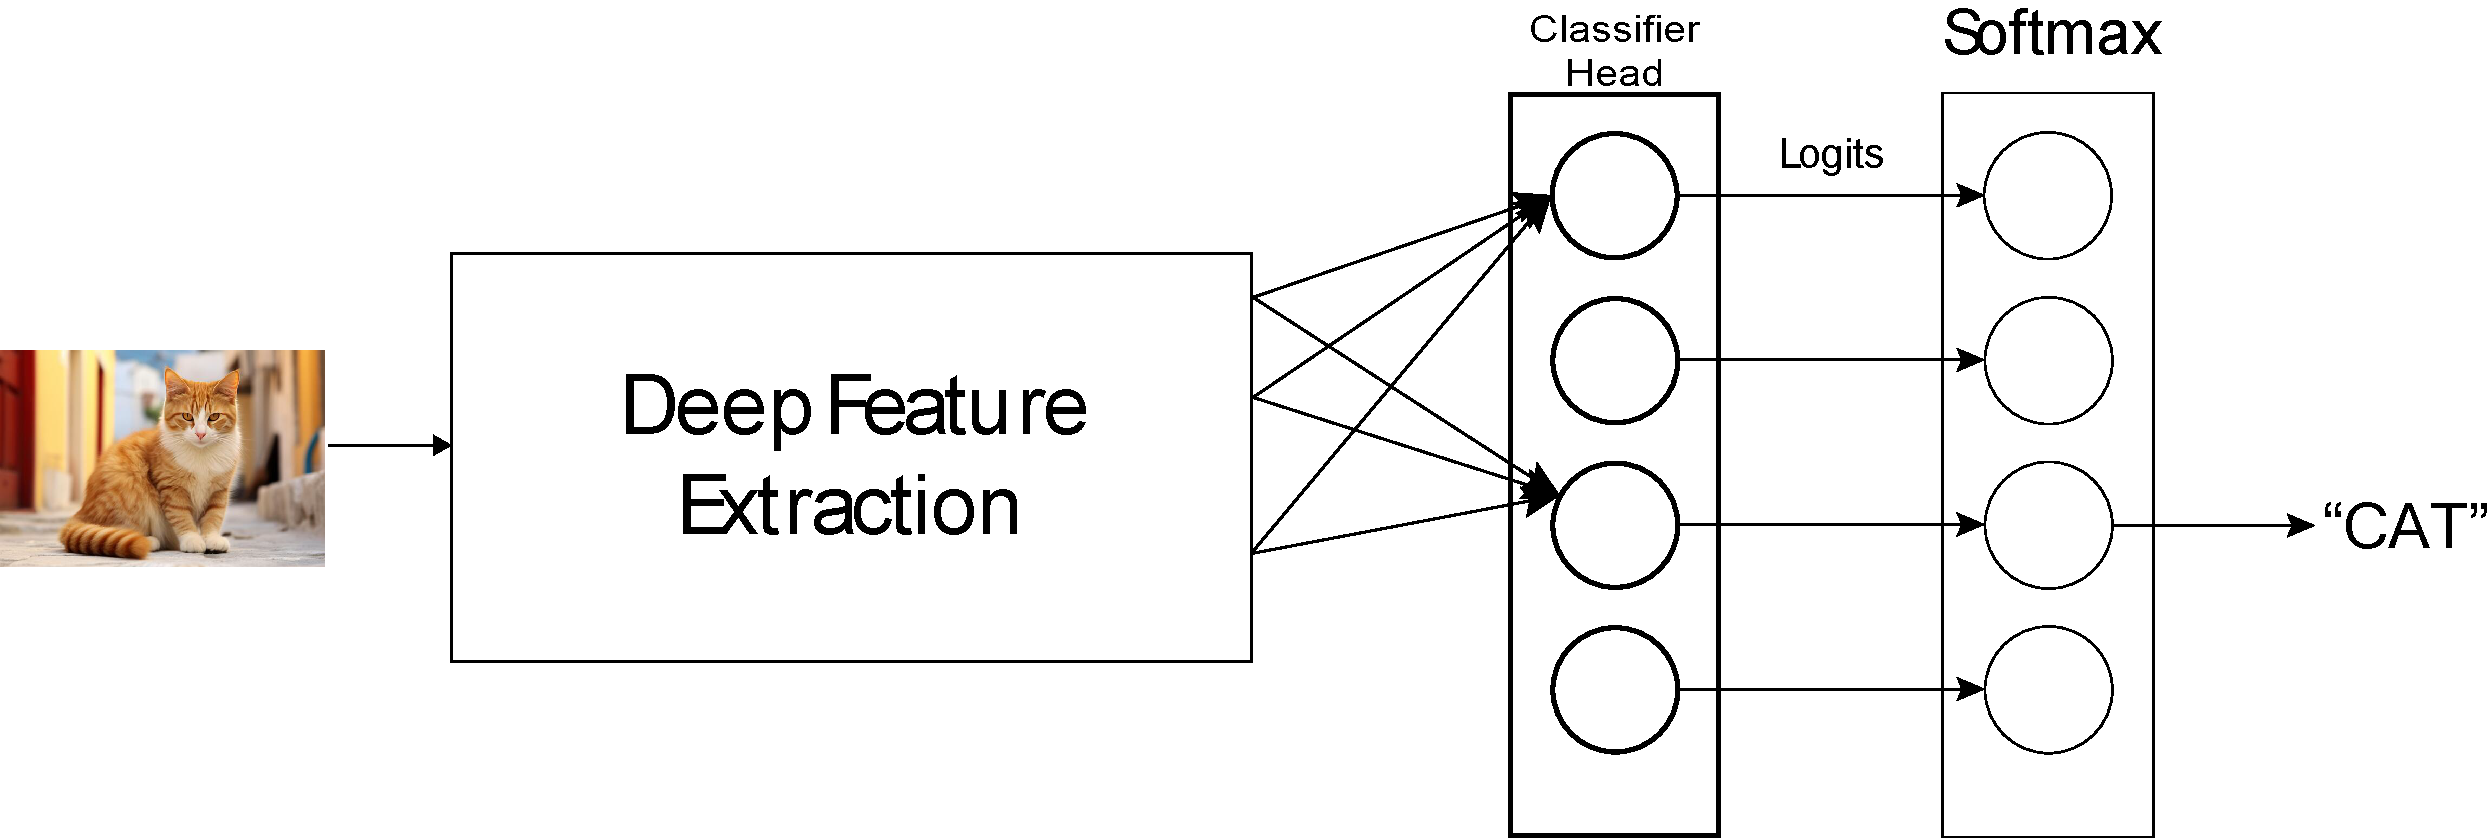
\includegraphics[width=0.8\textwidth]{basic-classification}}
    \caption{Basic Classification}
    \label{fig:basic_classification}
\end{figure}

In the \autoref{fig:basic_classification}, we can see a high-level overview of the basic classification task. The process can be summarized as follows:

\begin{enumerate}
    \item The input image is passed through the model, and the feature maps are generated. This deep feature extraction block can be either CNNs (as it initially was) or Transformers.
    \item The \emph{MLP (Multi-Layer Perceptron)}, also called the \emph{Classifier head}, is used to produce the final classification scores.
    \item The scores are then normalized using a \emph{softmax} function to obtain the class probabilities.
\end{enumerate}

No matter how the feature maps are generated or what the backbone is, the MLP head is used to produce the final classification scores. For CAM generation, we only need the feature maps and the class scores, i.e, upto the Classifier head.

Convolutional Neural Networks (CNNs) are often considered “black-box” models due to the limited interpretability of their internal decision-making process. To address this, Class Activation Mapping (CAM) was introduced by Zhou et al.~\cite{cam}, demonstrating that CNNs can act as unsupervised object detectors by highlighting discriminative image regions relevant to classification. CAM and its variants have since become central to Weakly Supervised Semantic Segmentation (WSSS), where such localization cues are refined into pixel-level pseudo-labels for segmentation training.

\subsection{Vanilla CAM}

The original CAM~\cite{cam} requires a specific network architecture where fully connected layers are replaced by a Global Average Pooling (GAP) layer followed by a linear classifier. The process is illustrated in \autoref{fig:basic_cam_generation_process}:

\begin{figure}[htbp]
    \centering
    \fbox{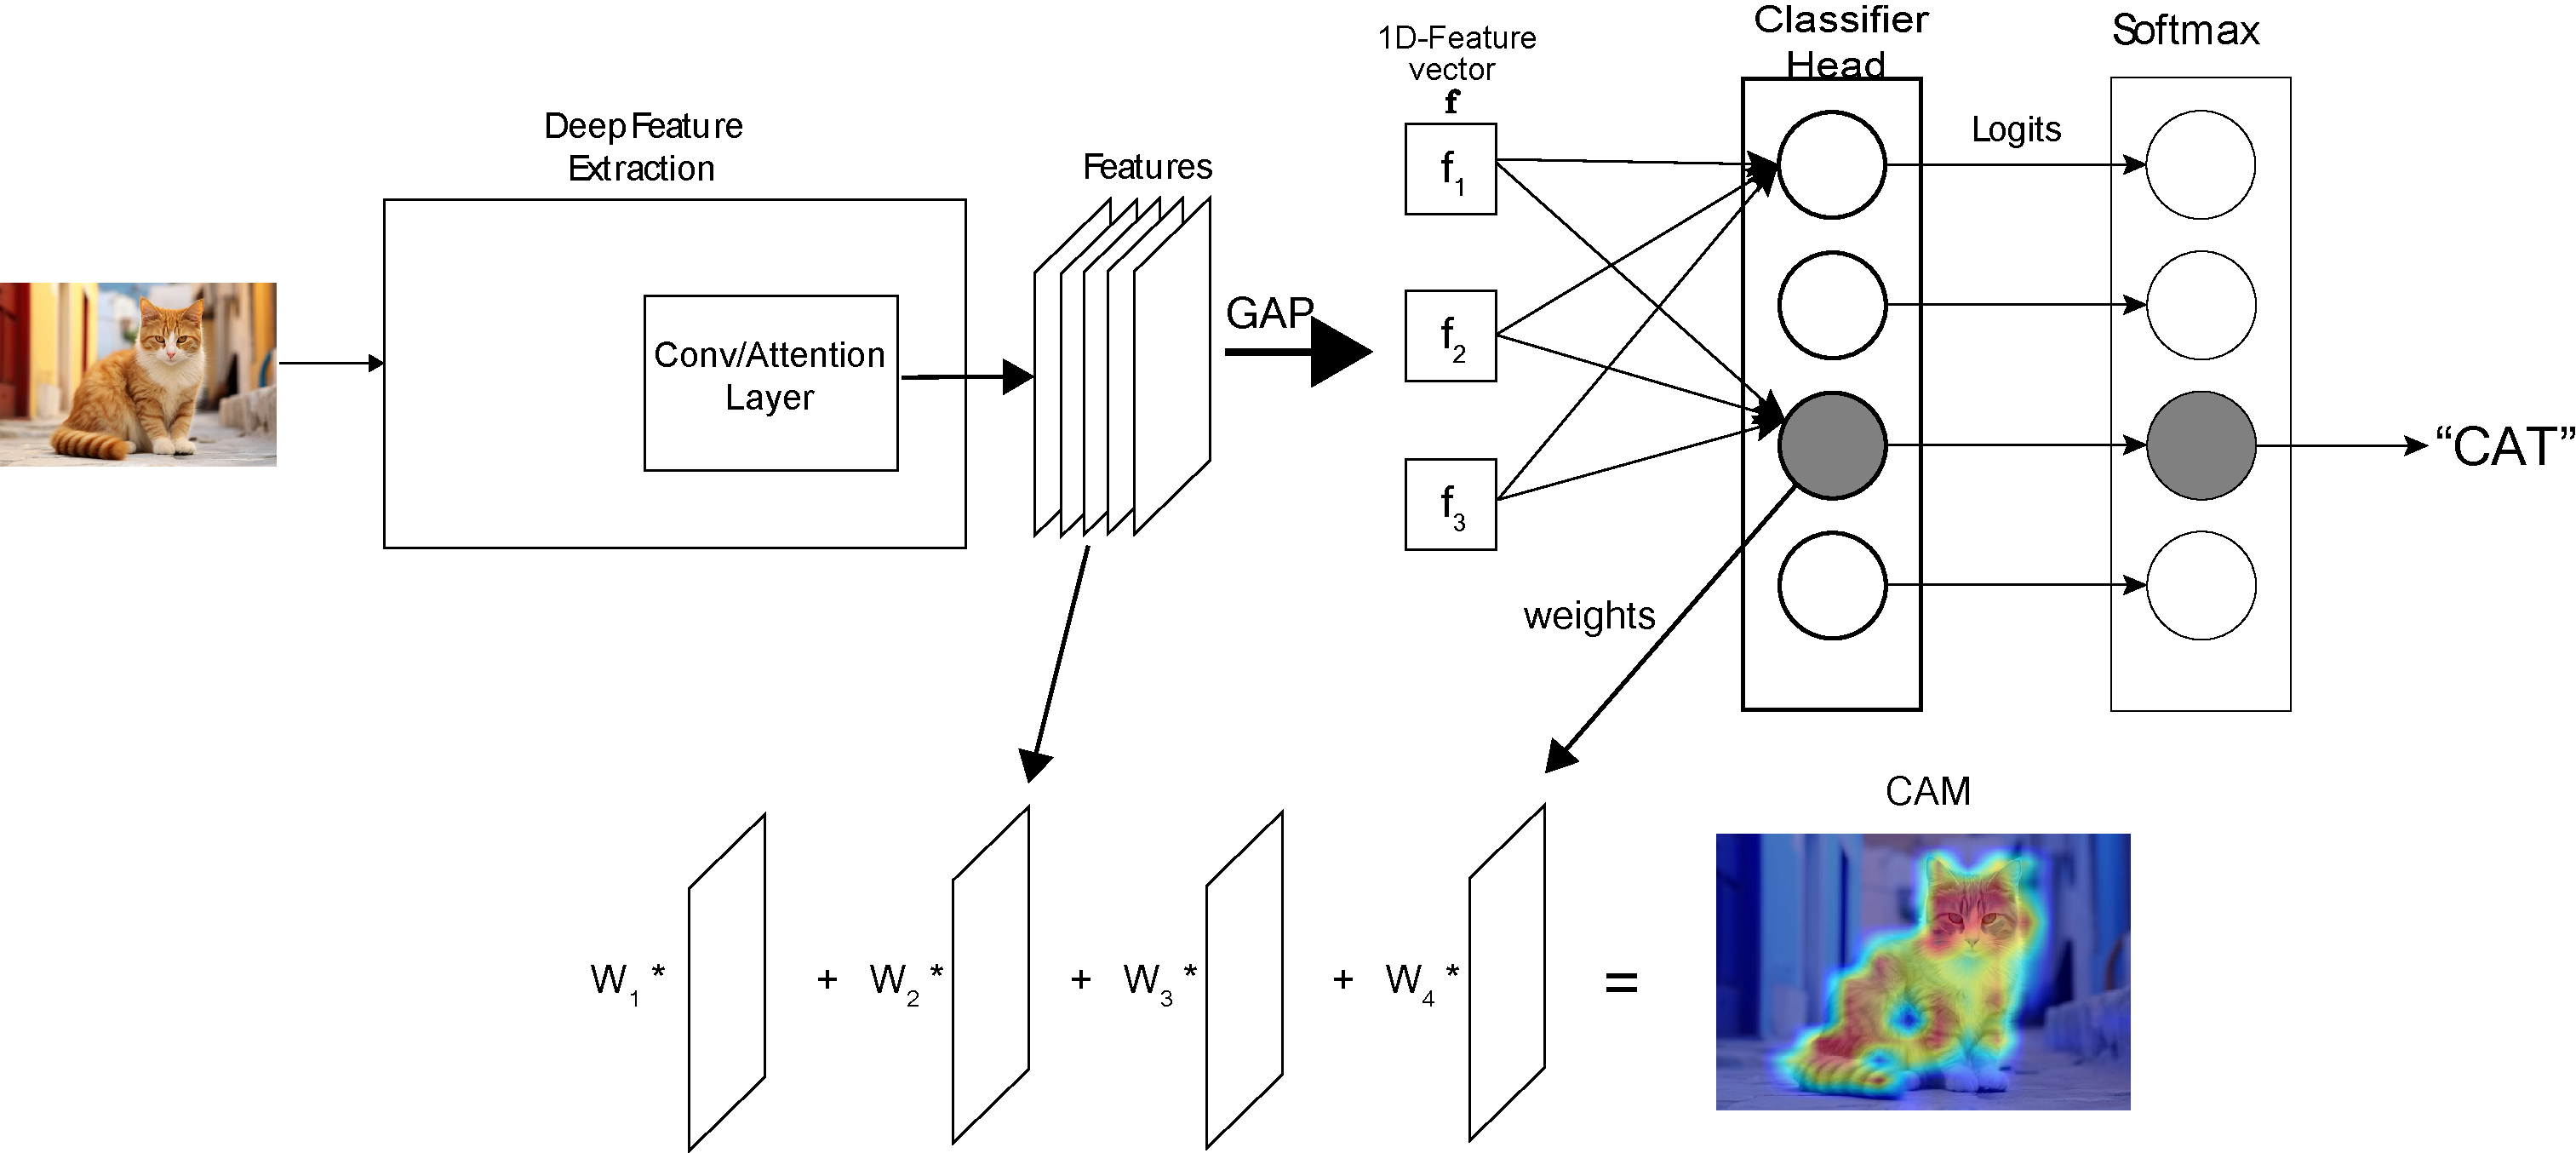
\includegraphics[width=0.8\textwidth]{basic-CAM}}
    \caption{CAM Generation Process}
    \label{fig:basic_cam_generation_process}
\end{figure}

\begin{enumerate}
    \item The input image is passed through a CNN to obtain convolutional feature maps.
    \item GAP is applied to produce a compact vector representation of the image.
    \item This representation is fed into the classifier head to generate class scores.
    \item The neuron corresponding to the predicted class is identified.
    \item The learned weights associated with this class are used to compute a weighted sum of the feature maps, yielding a class-specific heatmap.
    \item The heatmap is upsampled to match the original image resolution for visualization.
\end{enumerate}

Although effective, CAM requires modifying the network by inserting GAP, which limits its general applicability.

\subsection{Grad-CAM}
\label{subsec:grad_cam}

To overcome CAM's architectural constraint, Selvaraju et al.~\cite{cam_grad} proposed Gradient-weighted CAM (Grad-CAM). Unlike CAM, Grad-CAM can be applied to any CNN-based model without requiring structural changes. Instead of relying solely on classifier weights, Grad-CAM leverages the gradient of the target class score with respect to feature maps. The process is illustrated in \autoref{fig:grad_cam_generation_process}:

\begin{figure}[htbp]
    \centering
    \fbox{\includegraphics[width=0.8\textwidth]{grad-CAM}}
    \caption{Grad-CAM Generation Process}
    \label{fig:grad_cam_generation_process}
\end{figure}

\begin{enumerate}
    \item Forward pass the input to obtain feature maps from the last convolutional layer.
    \item Compute the classification scores through the classifier head.
    \item Select the target class neuron (often the top prediction, but any class can be chosen).
    \item Backpropagate to compute gradients of this class score with respect to the feature maps.
    \item Average the gradients spatially to obtain weights for each feature map channel.
    \item Combine the feature maps using these weights to create a coarse localization heatmap.
    \item Apply ReLU to suppress negative contributions.
    \item Upsample the heatmap to align with the input image.
\end{enumerate}

Grad-CAM preserves the architectural flexibility missing in CAM, while still providing class-discriminative localization.

\subsection{Grad-CAM++}
Grad-CAM++~\cite{cam_gradpp} was proposed to address two main limitations of Grad-CAM: (1) poor handling of multiple object instances of the same class, and (2) sensitivity to object size and distribution. Instead of relying only on first-order gradients, Grad-CAM++ incorporates higher-order derivatives of the class score with respect to feature maps.

\begin{enumerate}
    \item The forward pass generates feature maps as in Grad-CAM.
    \item For the target class, both first-order and higher-order gradients are computed.
    \item These gradients are used to calculate pixel-wise weights, where each spatial location contributes differently to the final importance score.
    \item The weighted sum of the feature maps is constructed using these refined weights, resulting in a sharper and more spatially precise heatmap.
    \item Like Grad-CAM, the heatmap is processed with ReLU and upsampled.
\end{enumerate}

This method improves localization in complex scenarios, such as small objects or multiple instances, while requiring only one backward pass, keeping computational costs similar to Grad-CAM.

\subsection{LayerCAM}
LayerCAM~\cite{layer_cam} builds on the intuition that meaningful localization is not limited to the last convolutional layer. Earlier and intermediate layers often capture fine-grained features such as edges and textures, which can complement coarse semantic features from deeper layers.

LayerCAM computes CAMs at multiple levels of the network:
\begin{enumerate}
    \item For each chosen convolutional layer, gradients with respect to the target class are calculated.
    \item Instead of spatially averaging the gradients, LayerCAM assigns weights at every spatial location by multiplying activation values with their corresponding gradients.
    \item These location-aware weights allow the method to produce more precise heatmaps per layer.
    \item CAMs from different layers are then combined to form a multi-scale localization map that captures both coarse object regions and fine details.
\end{enumerate}

By integrating multi-layer signals, LayerCAM enhances both interpretability and localization accuracy compared to Grad-CAM.

\subsection{Attention Rollout and Attention Flow}
Beyond CNN-based visualization, transformer-based networks introduced attention-based interpretability. Abnar and Zuidema~\cite{attention_rollout} proposed two techniques:

- \textbf{Attention Rollout}: recursively multiplies attention matrices across layers, incorporating residual connections. This assumes that token identity propagates linearly through attention weights, providing a global view of how input tokens influence the final decision.
- \textbf{Attention Flow}: formulates interpretability as a maximum flow problem, modeling information propagation as a flow network. A maximum flow algorithm is then applied to trace how embeddings in deeper layers are connected back to input tokens.

Both methods generate token-level importance maps that correlate strongly with gradient-based measures, improving interpretability for transformer architectures.

\subsection{RelevanceCAM}
RelevanceCAM~\cite{relevance_cam} incorporates Layer-wise Relevance Propagation (LRP) into CAM generation. Unlike gradient-based methods that can suffer from the shattered gradient problem, LRP redistributes the prediction score backward through the network based on relevance conservation principles.

\begin{enumerate}
    \item Starting from the target class score, relevance values are propagated layer by layer toward the input.
    \item Each neuron's contribution is quantified based on how much it supports the class prediction.
    \item These relevance scores are aggregated spatially to form heatmaps at multiple layers.
    \item The final activation map combines information from both shallow and deep layers, enhancing robustness and interpretability.
\end{enumerate}

RelevanceCAM provides more stable and faithful explanations, particularly in intermediate layers, and demonstrates improved localization performance over traditional Grad-CAM variants.

\subsection{Summary}
Overall, CAM-based methods have evolved from the original GAP-based CAM~\cite{cam} to gradient-driven approaches like Grad-CAM~\cite{cam_grad}, higher-order generalizations such as Grad-CAM++~\cite{cam_gradpp}, multi-layer extensions like LayerCAM~\cite{layer_cam}, attention-based methods for transformers~\cite{attention_rollout}, and LRP-driven methods like RelevanceCAM~\cite{relevance_cam}. These advances have been pivotal in WSSS, where class-discriminative heatmaps serve as initial localization cues that are refined into pixel-level pseudo-labels for segmentation.

\section{How WSSS models work: a breakdown}
\label{sec:how-wsss-models-work}

\subsection{Feature Extraction from Backbone}
\label{subsec:feature-extraction-backbone}

The architecture of AffinityNet \cite{wsss_affinitynet} relies on three DNNs: a classification network for generating CAMs, the AffinityNet module itself, and a segmentation network. All three share the same backbone. The backbone is a modified variant of Model A1 \cite{RevisitingResNET}, commonly referred to as ResNet38, which consists of 38 convolutional layers with wider channels. In this adaptation, the GAP and fully connected layers from the original design are removed, and the final three convolutional stages are replaced with atrous convolutions with stride 1. The dilation rates are adjusted so that the resulting feature maps maintain a stride of 8.

In DSRG \cite{wsss_dsrg_deep_seeded_region_growing}, the classification branch employs a slightly altered version of the 16-layer VGG model \cite{VGG16}, while the segmentation branch is built upon DeepLab-V2 \cite{fsss_deeplabv2}. Both are initialized with VGG-16 weights pre-trained on ImageNet.

AFA \cite{wsss_afa_affinity_from_attention} adopts the Mix Transformer (MiT) backbone introduced in SegFormer \cite{fsss_segformer}, which is more suitable for image segmentation tasks compared to the vanilla ViT. The MiT parameters are initialized using ImageNet-1k pre-trained weights.

ToCo \cite{wsss_toco_token_contrast} uses the ViT-Base (ViT-B) backbone initialized with ImageNet pre-trained weights. Within the ViT encoder, an auxiliary classification head is introduced to produce CAMs. These auxiliary CAMs are then used to form pseudo labels guiding the Pixel-Token Contrast (PTC) module, and also to generate proposals for cropping positive and negative local patches for the Cross-Token Contrast (CTC) module. The final CAM is generated through the classification layer and subsequently transformed into pseudo labels.

CLIP-ES \cite{wsss_clip_es} employs the CLIP ViT-B/16 backbone, where the image encoder extracts visual features and the text encoder extracts linguistic features. Since CLIP is pre-trained on roughly 400 million image-text pairs, it provides strong multimodal representations for segmentation.

The whole framework of FrozenCLIP \cite{wsss_frozen_clip} consists of four major components: a frozen CLIP backbone (comprising a ViT-Base/16 image encoder and a text encoder) \cite{transformer_vit}, a classification module for generating initial CAMs, a decoder for segmentation prediction, and a refinement module (RFM) to enhance CAMs into pseudo labels for supervision.

\subsection{CAM generation}
\label{subsec:cam-generation}
In AffinityNet \cite{wsss_affinitynet}, CAMs are generated by appending three layers to the backbone: a 3×3 convolutional layer with 512 channels for task adaptation, a global average pooling layer to aggregate spatial information, and a fully connected layer for classification. The class activation maps are computed by weighting the feature maps with the class-specific weights from the final layer. These maps are normalized such that their maximum value is 1, and the background map is obtained by subtracting the maximum class activation at each pixel from 1.

In DSRG \cite{wsss_dsrg_deep_seeded_region_growing}, CAMs \cite{cam} are used to localize foreground regions. The classification branch applies a fully connected layer to the conv7 features, producing a heatmap for each class. Foreground seed cues are extracted by thresholding these heatmaps, while background cues are identified from regions in normalized saliency maps with low pixel intensities.

AFA \cite{wsss_afa_affinity_from_attention} similarly employs CAMs to generate initial pseudo labels. These maps are formed by linearly combining feature maps from the classification layer using learned weights, followed by a ReLU activation to suppress negative values. The outputs are then scaled to the [0,1] range, and an additional background score is included to differentiate foreground from background.

ToCo \cite{wsss_toco_token_contrast} incorporates an auxiliary classification layer to extract semantic information and produce CAMs. Patch tokens are aggregated using global max pooling and subsequently passed through a fully connected layer, resulting in auxiliary CAMs that guide the model's training.

In FrozenCLIP \cite{wsss_frozen_clip}, image features are extracted from the frozen CLIP image encoder, while class-specific text prompts are processed by the CLIP text encoder, both remaining fixed during training. Classification scores are calculated as distances between pooled image and text features, and Grad-CAM \cite{cam_grad} is applied to these scores to generate the initial CAMs.


\subsection{Pseudo Label Generation}
\label{subsec:pseudo-label-generation}
AffinityNet predicts convolutional feature maps in which the semantic affinity between two feature vectors is measured using their L1 distance. To train this network, semantic affinity labels are derived from CAMs. Specifically, confident foreground and background regions are identified, while ambiguous regions are treated as neutral. Pairwise affinities are then defined according to class labels — assigned as 1 for pixels of the same class, 0 for different classes, and ignored for neutral labels. Once trained, AffinityNet refines CAMs through a random walk guided by the semantic transition matrix, thereby enhancing CAM quality and producing more accurate pseudo segmentation labels.

In DSRG, pseudo labels are generated by expanding initial seed cues into unlabeled regions using the classical Seeded Region Growing (SRG) algorithm \cite{srg}. For each class, the seed cues are visited in row first manner and its 8-connectivity neighborhood pixels are checked for similarity criteria. If they satisfy the criteria , those pixels are added to the set of seed cues for that particular class, and this process is repeated for every object class. The dynamically updated seed sets act as supervision, continuously refining pseudo labels during training.

The AFA module computes semantic affinities directly by linearly combining multi-head attention outputs through an MLP layer. To ensure matrix symmetry, the affinity matrix is summed with its transpose, under the assumption that nodes with the same semantics should be equivalent. Supervision is provided by pseudo affinity labels derived from refined CAMs: pixels are assigned to the class with the highest activation, and affinities are set positive if two pixels share the same class, otherwise negative. These pseudo affinity labels supervise the affinity prediction process. The learned semantic affinities are then used in a random walk propagation to refine the CAMs.

In ToCo, auxiliary CAMs are segmented into pseudo token labels by applying two background thresholds, categorizing tokens into reliable foreground, background, and uncertain regions. Positive token pairs are defined as those sharing the same label, while others are treated as negative. To counteract over-smoothing, the Patch Token Contrast (PTC) module maximizes similarity between positive pairs of patch tokens and minimizes it for negative ones. Additionally, the Class Token Contrast (CTC) module enforces consistency across entire object regions by aligning representations of global and local class tokens. Specifically, it reduces the gap between projected global class tokens and projected local tokens cropped from uncertain or background regions, thereby improving pseudo label quality.

\subsection{Segmentation prediction}
\label{subsec:segmentation-prediction}
In AffinityNet, the segmentation model is constructed by adding two atrous convolution layers on top of the backbone. The segmentation predictions are then supervised using refined CAMs, which are generated by propagating pairwise pixel affinities.
For DSRG, once seed cues are obtained from initial CAMs, an image semantic segmentation network is trained with these cues. A balanced seeding loss is applied so that the network's predictions are encouraged to match only the seed regions defined by the classification network, while ignoring unlabeled pixels. As training progresses, the seed cues are iteratively refined into pseudo labels, and the segmentation model is retrained with the updated supervision.
In ToCo, the segmentation decoder is deliberately simple, consisting of two 3×3 convolutional layers (each with dilation rate 5) followed by a 1×1 prediction layer. The pseudo labels produced by ToCo are passed through a Pixel-Adaptive Refinement (PAR) module, and the improved labels serve as supervision for the decoder to generate the final segmentation output.
For AFA, an MLP-based decoder head is employed. This head fuses features across multiple levels through lightweight MLP layers to produce segmentation predictions. The supervision is provided by refined pseudo labels obtained through affinity propagation.
In FrozenCLIP, segmentation is guided by a feature decoder that extracts intermediate outputs from each transformer block of the CLIP image encoder. For each feature map, a dedicated MLP is applied to generate enhanced feature representations, which are concatenated and then passed through a convolutional layer to form a fused feature map. This fused representation is subsequently processed by multiple stacked multi-head transformer blocks, producing the final segmentation prediction P.